% This LaTeX was auto-generated from MATLAB code.
% To make changes, update the MATLAB code and export to LaTeX again.

\documentclass{article}

\usepackage[utf8]{inputenc}
\usepackage[T1]{fontenc}
\usepackage{lmodern}
\usepackage{graphicx}
\usepackage{color}
\usepackage{listings}
\usepackage{hyperref}
\usepackage{amsmath}
\usepackage{amsfonts}
\usepackage{epstopdf}
\usepackage{matlab}

\sloppy
\epstopdfsetup{outdir=./}
\graphicspath{ {./ejercicio08_completo_images/} }

\begin{document}

\matlabtitle{Ejercicio N°8}

\matlabheading{Respuesta al impulso}

\begin{matlabcode}
syms C1 C2 C3 C4 C5 C6 s R1 R2 E1 v1 v2 v3 v4;
\end{matlabcode}

\begin{par}
\begin{flushleft}
La matriz de admitancias
\end{flushleft}
\end{par}

\begin{matlabcode}
Y=[1/R1+s*C1+s*C5 -s*C5 -s*C1 0; -s*C5 s*C5+s*C2+1/R2 0 -s*C2;-s*C1 0 s*C1+s*C3+s*C6 -s*C6;0 -s*C2 -s*C6 s*C6+s*C4+s*C2]
\end{matlabcode}
\begin{matlabsymbolicoutput}
Y = 
    $\displaystyle \left(\begin{array}{cccc}
C_1  s+C_5  s+\frac{1}{R_1 } & -C_5  s & -C_1  s & 0\\
-C_5  s & C_2  s+C_5  s+\frac{1}{R_2 } & 0 & -C_2  s\\
-C_1  s & 0 & C_1  s+C_3  s+C_6  s & -C_6  s\\
0 & -C_2  s & -C_6  s & C_2  s+C_4  s+C_6  s
\end{array}\right)$
\end{matlabsymbolicoutput}
\begin{matlabcode}
Is=[E1/R1;0;0;0]
\end{matlabcode}
\begin{matlabsymbolicoutput}
Is = 
    $\displaystyle \left(\begin{array}{c}
\frac{E_1 }{R_1 }\\
0\\
0\\
0
\end{array}\right)$
\end{matlabsymbolicoutput}
\begin{matlabcode}
x=[v1;v2;v3;v4];
Y\(Is)==x;
eqs=Y*x==Is;
solu=solve(eqs);
\end{matlabcode}


\begin{par}
\begin{flushleft}
Reemplazando los valores del circuito
\end{flushleft}
\end{par}

\begin{matlabcode}
C1=1;C2=2;C3=3;C4=4;C5=5;C6=6;R1=1;R2=1;E1=1;
\end{matlabcode}

\begin{par}
\begin{flushleft}
La función de transferencia $ H(s)=V2(s)/E(s)$
\end{flushleft}
\end{par}

\begin{matlabcode}
v2s=subs(solu.v2)
\end{matlabcode}
\begin{matlabsymbolicoutput}
v2s = 
    $\displaystyle \frac{432 s}{988 s^2 +1040 s+84}$
\end{matlabsymbolicoutput}

\begin{par}
\begin{flushleft}
La respuesta al impulso es
\end{flushleft}
\end{par}

\begin{matlabcode}
vpa(rewrite(ilaplace(v2s),'exp'),4)
\end{matlabcode}
\begin{matlabsymbolicoutput}
ans = 
    $\displaystyle 0.4372 e^{-0.5263 t}  {\left(1.101 e^{-0.4382 t} -0.1006 e^{0.4382 t} \right)}$
\end{matlabsymbolicoutput}

\begin{par}
$$v2(t)=0.4813 e^{-0.9645t}-0.04398e^{-0.0881t}$$
\end{par}


\matlabheading{Solución con Backward-Euler}

\begin{matlabcode}
clear all;
% Valores de los componentes
R1=1;R2=1;C1=1;C2=2;C3=3;C4=4;C5=5;C6=6;
% Matrices forma general
M=[C1*R1 0 C5*R1 0;-R2*C2 0 (C5*R2+R2*C2) -R2*C2; C1 -C3 0 -C6;C2 -C4 -C2 C6+C4+C2];
N=[1 1 0 0;-1 -1 1 0;0 0 0 0;0 0 0 0];
% Matriz forma normal
A=-1.*(M\N);
% Condiciones iniciales
v01=0;v02=0;v03=0;v04=0;v05=0;v06=0;
Xant=[v01;v03;v05;v06];

clear  t
solu=[];
ti=0;
tf=10;
h=0.1;
for t=ti:h:tf
    if t<=5
    E=(sin(0.2*pi*t))^2;
    else
     E=0;
    end
    u=[E;0;0;0];
     X=((((1/h).*M)+N)\u) + ((((1/h).*M)+N)\((1/h).*M)*Xant);
    solu=[solu X];
    Xant=X;
end
t=ti:h:tf;
\end{matlabcode}


\begin{matlabcode}
vr2=solu(1,:)+solu(2,:)-solu(3,:);
plot(t,vr2)
hold on;
\end{matlabcode}


\matlabheading{Solución convolución numérica}

\begin{matlabcode}
clear all;
syms t tau  
E= sin(pi/5*tau)^2*(heaviside(tau)-heaviside(tau-5));
imp=0.4813*exp(-0.9645*(t-tau))-0.0440*exp(-0.0882*(t-tau));
v2int=int(imp*E,tau,0,t);
fplot(v2int,[0,10])
hold off;

legend({'Euler','Convolución'})
title('Respuesta temporal VR2')
xlabel('tiempo [s]')
ylabel('Voltaje [V]')
\end{matlabcode}
\begin{center}
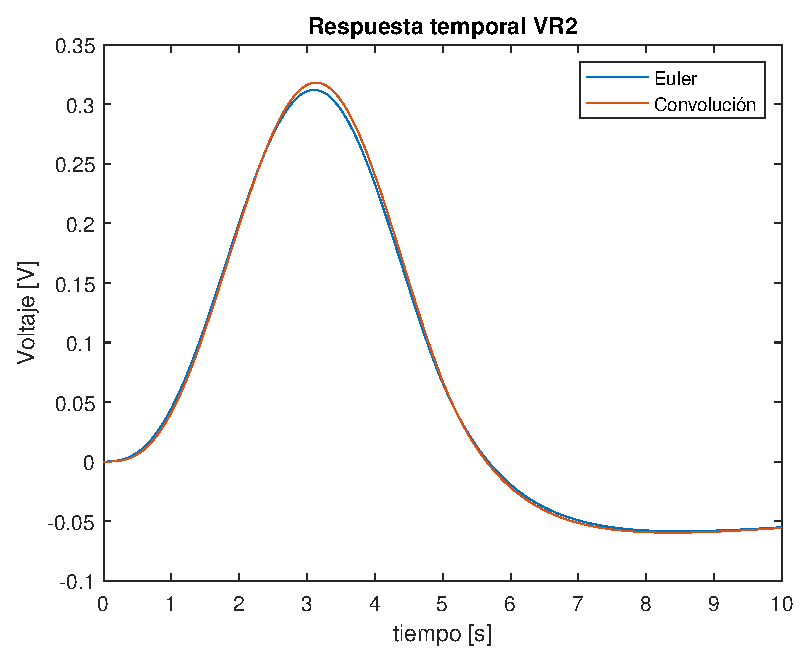
\includegraphics[width=\maxwidth{56.196688409433015em}]{figure_0_08}
\end{center}

\end{document}
